%\begin{savequote}[8cm]
%\textlatin{Jedem Anfang wohnt ein Zauber innne.}
%
%In the core of every beginning lives magic.
%  \qauthor{--- Hermann Hesse's \textit{Stufen}}
%\end{savequote}

\chapter{\label{ch:2-background}Theoretical Background} 

%\minitoc

\section{Introduction}
This chapter describes the theoretical background of machine learning and counterfactual inference including their formalisation, core concepts, state-of-the-art, and challenges. 

We start by giving a general introduction to machine learning and  its core concepts. 

The second part of the chapter deals with  \emph{deep learning} -- a particular subset of machine learning that uses deep neural networks. 

The last part of the chapter is dedicated to the problem of counterfactual inference. We describe the importance of the problem and its application areas, and give a formalisation. Furthermore, we outline the challenges of the problem and the different approaches that have been applied to it so far. We conclude, by relating counterfactual inference to deep learning and describing its open research questions which is the very foundation of this thesis. 

% TODO Intro: Write introduction in more detail depending on the actual contents. 


\section{Machine Learning}


\subsection{Motivation}
When conceptualising computer programs, we often think of them as series of unambiguous, (mostly) atomic instructions that are executed in a deterministic way and have to be explicitly programmed by a human programmer. 

While certain problem areas -- in particular those for which a well-defined algorithm or effective step-by-step solution strategy exists -- can successfully expressed and ultimately solved this way, there are various problems where this seems infeasible. A typical example for the second category is autonomous driving for which there are far too many situations and eventualities to encode the desired behaviour of an autonomous vehicle as a finite sequence of conditional instructions. 

Machine learning is a subfield of computer science that deals with the question of how to teach computer programs to learn without being explicitly programmed what to do. 
% TODO Check if this it too close to the quote at wikipedia 

More formally, an algorithm "is said to learn from experience E with respect to some class of tasks T and performance measure P if its performance at tasks in T, as measured by P, improves with experience E". (Mitchell)
% CITE:  Mitchell, T. (1997). Machine Learning. McGraw Hill. p. 2. ISBN 0-07-042807-7.
Recalling our example of autonomous driving, for instance, we could define the task $T$ in terms of "moving the car from A to B" while our performance measure $P$ might include aspects such as the travel time and the number of people or objects harmed. The experience $E$ would consists of the \emph{training data} that is acquired by previously covered distances (either autonomously or by "observing" a human driver). 

% TODO Show diagram (model, algorithm, learning, data)

\subsection{Types of Learning}
Machine Learning is typically categorised into \emph{supervised learning}, \emph{unsupervised learning}, \emph{reinforcement learning}. 

% TODO For each of the categories, make it more formal 

\subsubsection{Supervised Learning} 
In supervised learning the task is to infer a function over a number of samples from a set of training data that is said to be \emph{labelled}. In other words, for each sample in the training data, we have access to the actual function value we want to predict. 

For instance, we might be interested predicting housing prices where we are given a dataset consisting of historic information regarding houses (e.g. number of rooms, area in $m^2$, etc.), commonly referred  to as \emph{features} or \emph{covariates}, and the actual price for which the house has been sold, called \emph{outcome}, \emph{target}, or \emph{label}. Once a certain model has been trained by using the historic labelled dataset, we can use the same model to predict the housing prices on unseen data points, i.e. new houses for which the price is unknown. Such a task of predicting a continuous variable is called a \emph{regression} task whereas the predicting of a discrete output is referred to as a \emph{classification} task. 

\subsubsection{Unsupervised Learning} 
In contrast to supervised learning, the training set in an unsupervised setting does not contain the target labels. Typical tasks in this field include finding particular patterns in the data and clustering it accordingly. It is important to note, however, that for supervised learning, there is normally no ground-truth meaning that the performance (or quality) of the outcome cannot be easily be measure or even defined in absolute terms but might depend on the underlying use-case of the clustering. Another important task in supervised learning is \emph{dimensionality reduction} for which a (in terms of the features) high-dimensional dataset is reduces to a target lower dimension while trying to minimise the information loss. 

\subsubsection{Reinforcement Learning}
In reinforcement learning, a software agent has to learn appropriate actions in a dynamic environment in which the consequences of an action might not be immediately accessible but add up to a long-term reward that ought to be maximised. 

A most prominent example was mentioned earlier with the task of autonomous driving in which a vehicle is governed by a piece of software that has to find adequate series of actions (steering, regulating speed, etc.) in order to reach a target destination in a complex and ever-changing environment. 


% TODO! Re-create graph!
\begin{figure}[]
	\caption{Schematic Approach of Machine Learning. A selected model $M$ is trained on a dataset $D$ using a learning algorithm $A$.} \label{fig:machine-learning-approach}
	\centering
	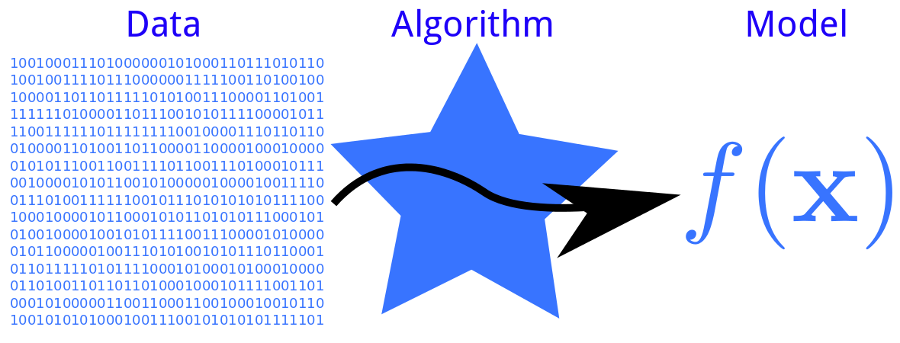
\includegraphics[width=0.5\textwidth]{figures/chapter-2/machine-learning-approach.png}
\end{figure}
\subsection{Machine Learning Models}
As illustrated in figure \ref{fig:machine-learning-approach}, machine learning is based on the concept of selecting an appropriate model and fitting it to a given (training) data set using a training algorithm. 

For instance, we might want to use a \emph{linear model} for our task of predicting housing prices. We can then make use \emph{linear regression} which allows us to fit our linear model to our labelled dataset of existing houses and their prices. 
 
The selection of an appropriate model is of great importance and determines important factors such as the trade-off between the expressiveness (i.e. the ability to capture complex relationships) and the computational complexity of our model (i.e. how difficult it is to train it). 

There is a number of models each with individual pros and cons depending on the desired task and the desired characteristics. Typical models include \emph{linear models}, \emph{decision trees}, and \emph{neural networks}. 
% TODO What are other typical models. How do they compare against each other? 
% Should I sketch them out here? 

This dissertation focuses on using \emph{deep learning} for the problem of counterfactual inference. Therefore, a dedicated part of this chapter deals exclusively with deep neural networks and describes their characteristics in more detail. 



%\subsection{Training}
%Machine learning is based on the concept of training a selected model by using a 
%
%Typically: Gradient Descent
%
%
%What types are there? 
%What's the challenge? (local minimum, symmetries, etc.)
%% TODO Include graph

\subsection{Regularisation} \label{sec:regularisation}
When training our model we have to find the right balance between fitting it most accurately to the training data while making sure that the model generalises will for unseen data points. 
Given that the expressiveness of the model is sufficiently high to capture it, we might naively fit our model to the training data perfectly, resulting in a training error of zero. This, however, would merely "memorise" the training data and might perform poorly on unseen future data points. This phenomenon where we overfit the training data is often referred to as \emph{high variance}. 
In contrast, if the model is too simple, we night not be able to accurately capture the relationship in our data leading to equally poor results. In this case, we are under-fitting the data and our model has a so called \emph{high bias}.
Therefore, the goal is to train the model in a way that neither overfits nor underfits and generalises well to unseen datapoints. This can be achieved by a concept called \emph{regulariation}.

% TODO Add formula for objective functions with L1 and L2 regularisation

% TODO Regularistion is actually just for avoiding overfitting!   

% TODO! Re-create graph!
\begin{figure}[]
	\label{fig:overfitting-underfitting}

	\centering
	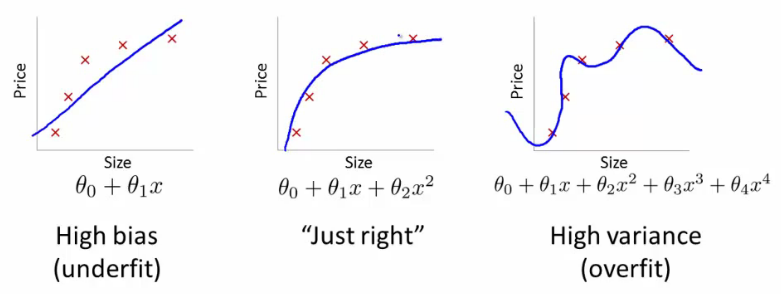
\includegraphics[width=0.8\textwidth]{figures/chapter-2/overfitting-underfitting.png}
	\caption{Visualisation of Bias variance Tradeoff. The model on the left is ... whereas the middle one ... and the right one is ...}
\end{figure}

% TODO Should I include learning curves as well? 
%% TODO! Re-create graph!
%\begin{figure}[]
%	\label{fig:machine-learning-approach}
%	\caption{Visualisation of Learning Curves. The left model is ... whereas the right model is ...}
%	\centering
%	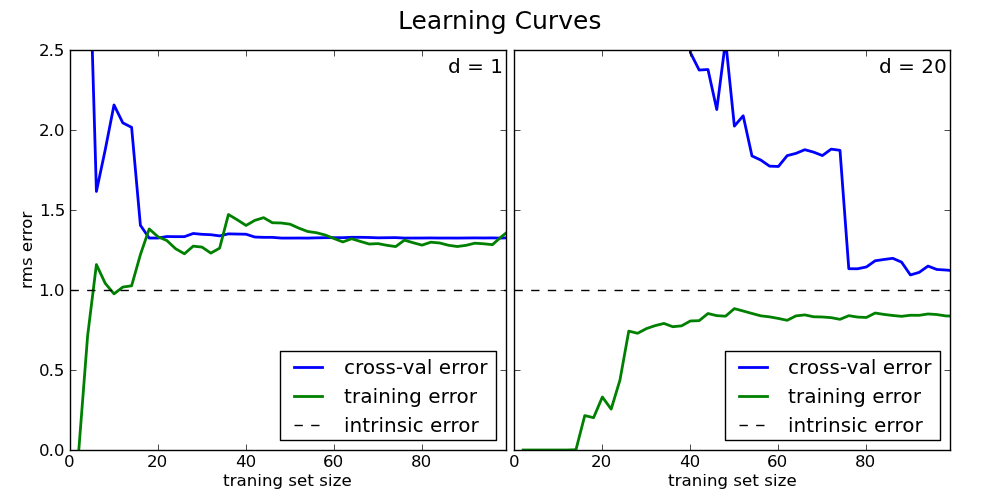
\includegraphics[width=0.8\textwidth]{figures/chapter-2/learning-curves.png}
%\end{figure}




\section{Deep Learning}
\subsection{Introduction}
Deep learning refers to a field of machine learning that is based on the use of so called \emph{deep neural networks}. 

The approach is inspired by how the human brain works by modelling biological neurons and their interconnections to other neurons as terms of an artificial neuron that has similar properties. 

The details about our understanding of the inner mechanics and biochemical processes of the human brain are beyond the scope of this thesis. On a high level, however, Each neuron receives inputs signals on its dendrites which are connected to neighbouring neurons axons using a synapse. The inputs are accumulated and processed within the cell body causing the cell to output a signal on its own axon which in turn represents the potential input for other cells.
% TODO Refine this. Make sure this is correct and in the right section! What exactly is a synapse. 
Through these interconnections the neurons form a highly complex structure that can be conceptualised in terms of a biological neural network. It is estimated that the human brain possesses about 100 billion allowing it to process complex signals, abstract concepts, and the general process people refer to as \emph{thinking}. 
% TODO What about learning? 

In a bionic fashion an artificial neural network adopts this architecture in a simplified way by defining a network of artificial neurons that are connected according to a certain topology. The analogy between the human and the artificial neurons is illustrated in figure \ref{fig:biological-vs-artificial-neuron}. 
This way, an artificial neural network (henceforth called neural network), is able to capture complex correlations and interdependencies within the data. 

% GRAPH Recreate graph
\begin{figure}[h]
	\caption{A biological neuron vs. an artificial neuron}\label{fig:biological-vs-artificial-neuron}
	% GRAPH-LABEL Add proper description
	\centering
	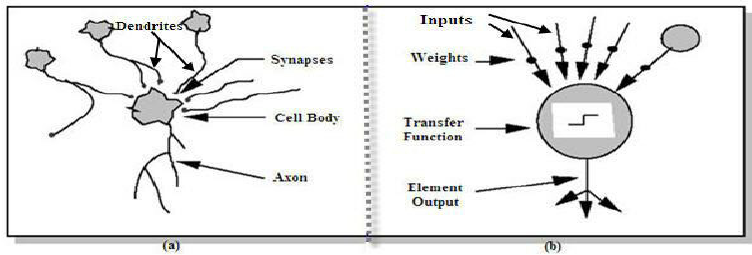
\includegraphics[width=0.8\textwidth]{figures/chapter-2/biological-vs-artificial-neurons.png}
\end{figure}


The concepts of using neural networks has been in existence since the 1970s. % CITE first neural networks
After an initial enthusiasm, however, neural networks lost traction in the following two decades due to the realisation that the existing hardware did not allow for a degree of scalability that would have been required to solve the desired problems. % CITE ai-winter

This changed, however, when in 2014 X,Y, and Z used a neural network outperformed all existing methods on the \emph{ImageNet Challenge} which seeks to recognise and label a set of objects in pictures. % CITE imagenet

Ever since, deep neural networks have been responsible for some of the most recent successes including self-driving cars and defeating the world champion in Go. % CITE Go 
According to former chief data scientist and researcher at Stanford University, Andrew Ng, % CITE Andrew Ng 
two key factors are responsible for renaissance of neural networks and have enabled its recent success: Firstly, the advances in computational capacities which includes highly-optimised processing units such as GPUs and ASICS % CHECK ASICS? 
and corresponding architectures such as distributed clusters and cloud computing. Secondly, the availability of large datasets that can be used for training the models such as web-scale text corpora for natural language processing or large databases of images (imagenet) etc. 

Today, deep neural networks represent the state-of-the-art in many areas such as natural language processing % CITE NLP
and computer vision. They are widely considered one of the most promising areas of machine learning and artificial intelligence in general % CITE importance of deep learning
and have received a high level of attention in society, media, and politics. Despite its recent success, the usage of deep neural networks poses a multitude of computational, architectural, and domain-specific challenges % CITE Do I need to cite this? 
and therefore represents of most dynamic areas of research. 

\subsection{The Multilayer Perceptron}
In order to understand how neural networks work, we first investigate one of the most basic forms of neural networks: the \emph{multilayer perceptron} or MLP. 
% TODO Is a perceptron the same thing as a neuron? Are there other kinds of neurons? 
% GRAPH Redo graph
\begin{figure}[H]

\caption{Prototypical multilayer perceptron with a single hidden layer.}\label{fig:multilayer-perceptron}
% GRAPH-LABEL Add proper description
\centering
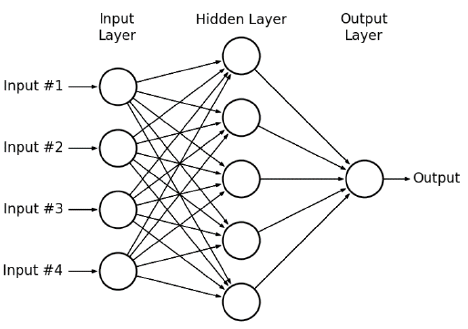
\includegraphics[width=0.6\textwidth]{figures/chapter-2/multilayer-perceptron.png}
\end{figure}
Figure \ref{fig:multilayer-perceptron} depicts the schematics of an MLP. As the name suggests, it consists of multiple layers each containing a fixed number of artificial neurons that are interconnected exclusively by neurons of neighbouring layers. The first, so called \emph{input layer}, is followed by one or more hidden layers leading to a final so called \emph{output layer}. 

\begin{figure}[h]
	\caption{Basic building block: Artificial Neuron used for classification.}\label{fig:artificial-neuron}   
	\centering
	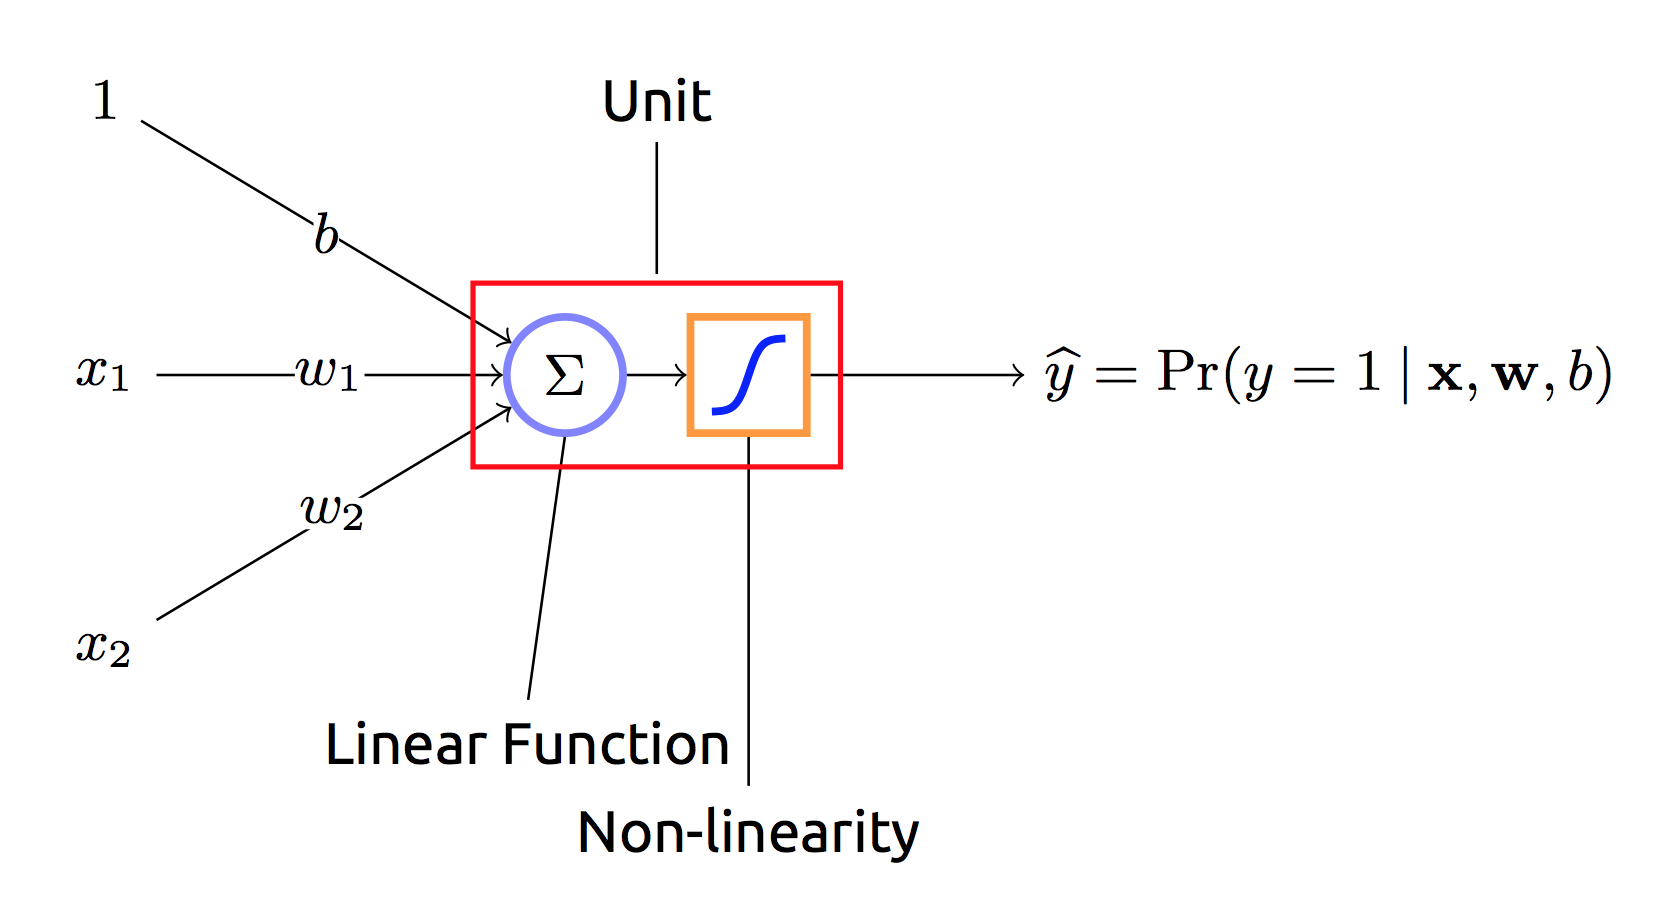
\includegraphics[width=0.6\textwidth]{figures/chapter-2/artificial-neuron.png}
\end{figure}


The individual artificial neuron or unit is illustrated in figure \ref{fig:artificial-neuron}. Its output $y$ is computed as 
\begin{equation}
	% MATHS Check, looks weird with b in front
	y = \phi(b + \sum_{i=1}^{n} w_i x_i)
\end{equation}
where $x_1, \ldots, x_n \in \mathbb{R}$ corresponds to the inputs of the neuron, $w_1, \dots, w_n\in \mathbb{R}$ to the weights and $b \in \mathbb{R}$ to a bias -- trainable parameters of the model -- and $\phi: \mathbb{R} \rightarrow \mathbb{R}$ to a non-linear function referred to as \emph{activation function}. Typical choices for $\phi$ include 
\begin{align*} 
\phi(x) = \sigma(x) = \frac{1}{1 + e^{-x}} && \text{or} && \phi(x) = tanh(x) = \frac{1  - e^{-2x}}{1  + e^{-2x}}
\end{align*} 
where $\sigma(x)$ refers to the \emph{sigmoid function}, $tanh(x)$ to the \emph{hyperbolic tangent}, and 
% TODO Add another activation function
... to Z. While each of these activation functions has different properties as illustrated in figure \ref{fig:activation-functions}, a typical characteristic is that they map the input value to the closed interval $[0, 1]$. 

\begin{figure}[h]
	\caption{Typical Activation functions}\label{fig:activation-functions}   
	\centering
	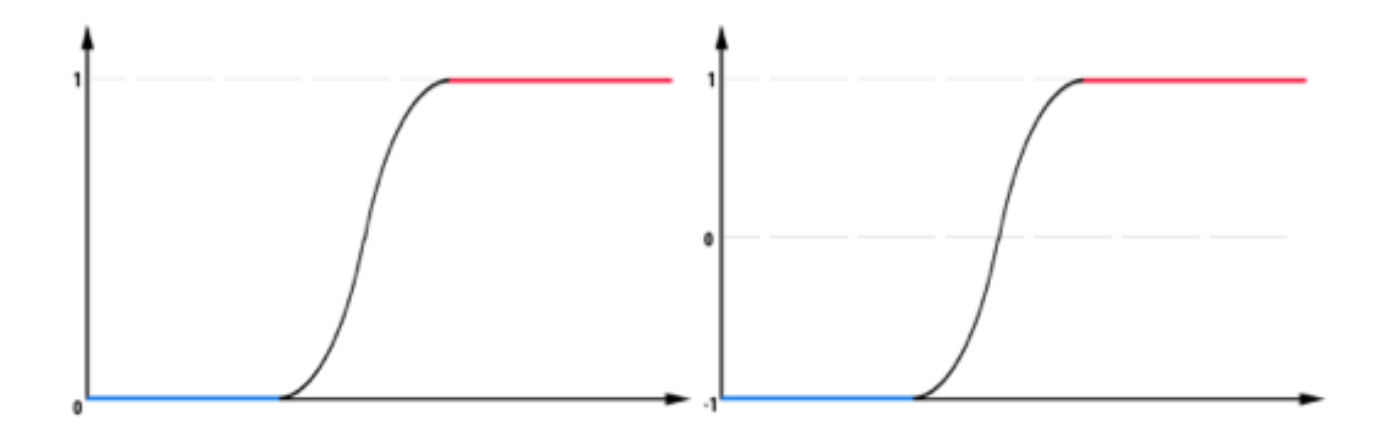
\includegraphics[width=0.6\textwidth]{figures/chapter-2/activation-functions.png}
\end{figure}


% TODO What else do I need to write about MLPs?  Equations for the outcome? 
%Given this definition of a single unit, the final value $y$ of the outcome layer can be formalised as the concatenation of the different activation functions forward-propagated from the input layer to the output layer. For the MLP depicted in figure \ref{fig:multilayer-perceptron}, this means.
%
%\begin{align}
%x = 
%\end{align}

Despite the relative simplicity of this model, it can be shown that an MLP with appropriate weights and bias parameters is able to represent any arbitrarily complex non-linear function.% CITE Who showed this? Cybenko!

\subsection{Types of Neural Networks} \label{sec:nn-types}
There are different types of neural networks defined by a number of characteristics such as network's architecture and the direction of information flow. 

% QUESTION: What's the difference between MLP and standard ff nn? 
\paragraph{Feed-Forward Neural Networks} Closely related to the MLP described in the previous section, feed-forward neural networks (FFNN) represent a class of networks that is characterised by a set of hidden layers that have a similar shape and are often fully connected (i.e. every node in layer $L_i$ is connected to every node in layer $L_{i-1}$ and $L_{i+1}$). As the name suggest, the information flow is strictly uni-directional from nodes in layers with lower indexes to nodes with higher indexes (i.e. no loops). These types of networks represent the most basic type of network that makes no assumptions about the input data and is used in regression and classification tasks.  

\paragraph{Convolutional Neural Networks} While FFNNs make no assumptions about the input data whatsoever, it is often useful to exploit domain-specific knowledge about the specific input data. For instance, in computer vision the input of a network is typically an image encoded as pixmap with the intensity values of each pixel. In this case, it seems naive and inefficient to assume independence of the inputs ignoring aspects like the principle of locality of neighbouring pixels which are more likely to have a similar colour or intensity than two randomly-selected pixels. 
% ALT: In contrast to FFNNs which make no assumption about the input whatserver, Convnets are designed to exploit domain-specific knowledge. In computer vision for instance, we can ... 
\begin{figure}[h]
	\centering
	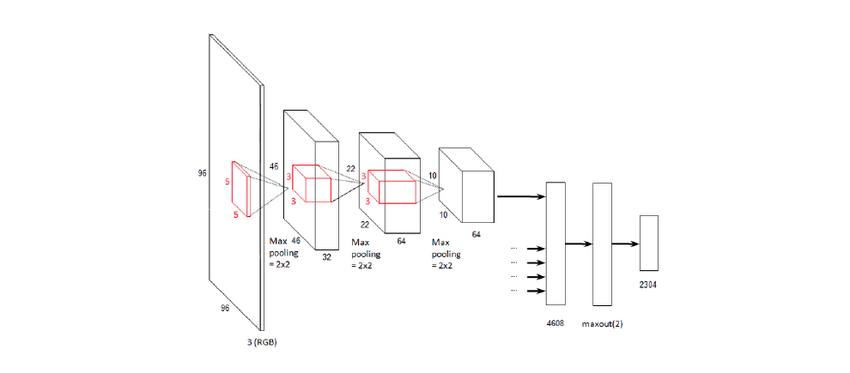
\includegraphics[width=1\textwidth]{figures/chapter-2/convnet.png}
	\caption{Convolutional Neural Network}\label{fig:convnet}   
\end{figure}
A convolutional neural network or ConvNet is a special kind of feed-forward neural network whose architecture is designed to exploit the principle of locality in the data. This is typically achieved by alternating \emph{convolutional layers} and \emph{pooling layers}. The convolutional layers run a filter or \emph{kernel} across the their input layer which performs an image convolution and can be thought of a way to detect features (such as edges) in the image. The pooling layers typically perform some kind of aggregation (such as taking the maximum of multiple values) over the previous layer to reduce the dimensionality. 

While convnets are particularly useful in computer vision and represent the state-of-the-art in image classification % CITE imagenet
, they can also be applied in other fields in which the data expresses some principle of locality. 

\paragraph{Recurrent Neural Networks} In contrast to FFNNs and convnets for which the information flow is strictly uni-directional, recurrent neural networks (RNNs) are characterised by some kind of feedback loop that allows the outputs of a unit in layer $L_i$ to be process as input by any other layer $L_j$, even if $i \geq j$.

This allows the network to keep an internal state which can be conceptualised as memory. Such a memory enables the network to effectively deal with sequences of data such as time-series values, natural language, or even music. 


\begin{wrapfigure}{r}{0.4\textwidth}
	\centering
	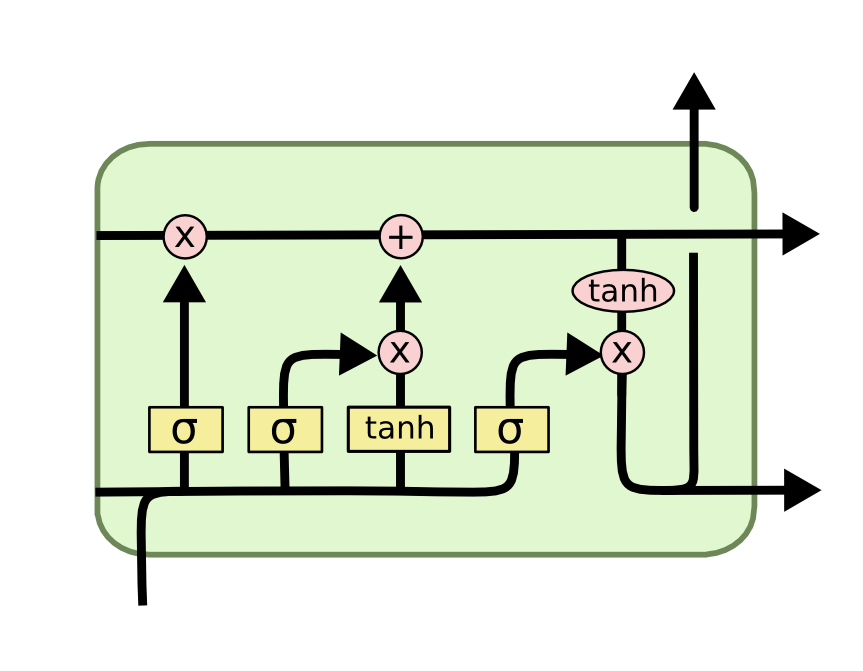
\includegraphics[width=0.4\textwidth]{figures/chapter-2/lstm.png}
	\caption{LSTM}\label{fig:lstm}   
\end{wrapfigure}

In spite of the benefits the recurrent architecture of the network provides, it also introduces a number of computational challenges such as the so called \emph{vanishing gradient problem} which stems from the additional distance the gradient is backpropagates (see next section % TODO Reconsider training section. Should it come before? 
) in the computation graph of the network causing the gradient. In order to circumvent this problem, a number architectures has been proposed for an individual cell within the RNN, most notably \emph{long short-term memory} (LSTM) cells and \emph{gated recurrent units} (GRUs). As illustrated in figure \ref{fig:lstm} an LSTM achieves this using a number of \emph{gates} that allow the cell to decide when to store and when to reset (i.e. forget) its internal state. 
% TODO Explain this properly. Make sure I fully understand it myself. ;) 

Today for many problems in machine learning, RNNs represent the state-of-the-art when dealing with sequential data such as natural language and time-series. 



\subsection{Training}
Training a neural network refers to the process of fitting the parameters of the model (i.e. the weights and bias for each cell) to the training data with respect to a given objective function. 

\paragraph{Objective Function}
\begin{wrapfigure}{r}{0.4\textwidth}
	\centering
	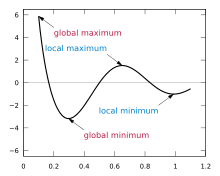
\includegraphics[width=0.4\textwidth]{figures/chapter-2/local-minima.png}
	\caption{Local Minima}\label{fig:local-minima}   
\end{wrapfigure}

The objective function (also called \emph{loss function} or \emph{error function}) defines a metric of the performance of the model. It is the goal of the training procedure to appropriate parameters for the model that maximise the performance or minimise its loss respectively. 

Figure \ref{fig:local-minima} illustrates this concept by depicting the graph of an objective function $f$ that takes a one-dimensional input (real numbered scalar). As we can see, the function posses multiple extreme values -- in particular one local minimum at $x = ?$% TODO add proper position
and a global minimum at $x = ?$. % TODO add proper position. 


In cases where an algebraically obtained closed-form solution for the minimum is not feasible or too computationally expensive, the minimum is often obtained by optimisation algorithms (see below). Since these algorithms often operate in a greedy manner, i.e. by a series of local operations that has no knowledge about the global surface of the function, we are facing the potential problem of only finding a local optimum but missing out the global one. As a consequence, it is desirable to use convex objective function that, by definition, only have one (global) minimum. 
The actual loss function is dependent on the problem task and can be derived by a maximum likelihood estimation (MLE). For regression tasks, a common choice is the mean squared error between the prediction $\hat{Y}$ and the actual output value $Y$ defined as 


\begin{align} 
L_{MSE}(w,b) = \frac{1}{n} \sum_{i=1}^{n}(\hat{Y}_i - Y_i)^2.
\end{align} 
For (binary) classification problems we typically use the cross-entropy
\begin{equation}
	L_{CE}(w,b) = - \frac{1}{n} \sum_{i=1}^{n} (Y_i \log \hat{Y}_i + (1 - Y_i) \log 
	(1- \hat{Y}_i)
\end{equation}
as loss function. 

\paragraph{Gradient Descent} We typically make use of an optimisation algorithm that tries to minimise the output of our loss function that captures the degree to what extend our prediction differs from the target values. A widely used example is \emph{gradient descent} which is an iterative optimisation algorithm that can be used to find a minimum value of a function. This is achieved by repeatedly computing the gradient of the function at the current position and subtracting a proportion of the gradient from it until the gradient converges towards zero (which is the case at a minimum) or a stopping condition is satisfied. Intuitively, the subtraction of the gradient can be conceptualised by taking iterative steps towards the steepest descent until a minimum value is reached. 
Formally, we are looking for $x = \text{argmin} f(x)$ by iteratively computing

\begin{equation}	
	\label{eq:gradient-descent-update}
	x_{n+1} = x_n - \alpha \cdot \nabla f(x_n),
\end{equation}
where $x_i$ refers to our position at time iteration $i$ and $\alpha \in \mathbb{R}^+$ is a parameter called the \emph{learning rate} that defines the step size of our descent. Choosing an appropriate learning rate typically represents a trade-off between reducing the number of required iterations (high learning rate) and a making sure the function converges and does not overshoot the actual minimum $x^*$ or oscillates around it. Consequently, it is often desirable to use an \emph{adaptive learning rate} instead, i.e. making $\alpha: \mathbb{N} \rightarrow \mathbb{R}^+$ a function of the current iteration. 

There two main types of gradient descent: \emph{batch gradient descent} computes the gradient for entire dataset before applying an update rule as defined in equation \ref{eq:gradient-descent-update} which is most exact but computationally expensive as it has to iterate through all $n$ data points in the dataset. In contrast, \emph{stochastic gradient descent} computes the gradient of a random (hence the name) sample and applies an update according to this sample alone which is less computationally expensive. The choice between the batch gradient descend and stochastic gradient descend therefore represents a trade-off between accuracy and computational costs. In addition to this dichotomy, there there exists a hybrid version called \emph{minibatch gradient descent} which computes the gradient on a batch which is a subset of the entire dataset. 

\paragraph{Backpropagation} For gradient-based optimisation algorithms it is mandatory to compute the partial derivatives of the objective function $J$ with respect to any weight $w$ or bias $b$ in the neural network that needs to be learnt. In a deep neural network with multiple hidden layers this might seem rather complex as change of weights influences the outcome (and therefore the loss function) only indirectly by propagating its change through subsequent layers. 

In the 1980s, X, Y, and Z % TODO Add history and contribution of backprop. Who invented it? When was it popularised? 
introduced an efficient method to achieve this which they called the \emph{backpropagation algorithm}. The algorithm conceptualised the network as a concatenation of functions and is based on the simple idea of repeatedly applying the \emph{chain rule} as known in calculus to compute the partial derivatives with respect to each parameter (weights and biases) of interest. 


\begin{wrapfigure}{r}{0.4\textwidth}
	\caption{Backpropagation}\label{fig:backpropagation}   
	\centering
	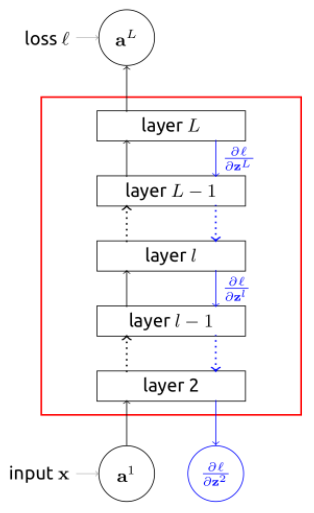
\includegraphics[height=0.6\textwidth]{figures/chapter-2/backpropagation.png}
\end{wrapfigure}


The training is then executed in two alternating phases as illustrated in figure \ref{fig:backpropagation}: In the \emph{forward pass} the inputs are propagated through the network from the input layer through the hidden layers until a predicted outcome $\hat{Y}$ is available in the output layer. Using the predicted outcome $\hat{Y}_i$, the actual outcome $Y_i$, and the loss function we are able to compute a loss \emph{l}.
In the second phase -- the \emph{backward pass} the partial derivatives are computed for the weights and biases of each unit all the way back until the first layer after the input layer. 

Once the partial derivatives are computed, we can update each parameter according to our optimisation algorithm (e.g. using gradient descent as described above). 
The backpropagation algorithm therefore represents an effective mean to compute the gradient of the loss function and can be considered an essential part of the training of neural networks. 



% TODO Check if should include any of the things below
%
%
%\begin{enumerate}
%	\item What does training mean? What is the main principle? We want to learn parameters (weights+bias). 
%	\item Backpropagation. History, when was it discovered? How does it work on high-level? What does each pass do? 
%	\item Explain splits train, test, val
%	\item Equations... Formalisation
%	\item Challenges (symmetry, local optima, initialisation, complexity, memory)
%\end{enumerate}

\subsection{Dropout}
As described in section \ref{sec:regularisation}, regularisation is an important concept in machine learning in order to avoid overfitting the training data. While in theory, a traditional approaches like \emph{l1} (lasso) and \emph{l2} (weight-decay) are possible, a number of different regularisation techniques have been proposed that are specific to the mechanics of neural networks. 

One of the most-used approaches is called \emph{dropout} and was proposed by % CITE Hinton
in 2014. The basic idea is that during training every neuron is kept active only with a certain probability $p$. With a probability of $1-p$ it represents an output of zero otherwise. Intuitively, this prevents the network from becoming too dependent on a particular neuron as it is forced to learn an alternative representation when it is disabled. As a consequence, the network learns a representation that generalises better giving dropout a regularising influence on the network. Similar to the regularisation hyper-paremeter $\lambda$ described in \ref{sec:regularisation}, the dropout probablity $p$ represents a hyper-parameter that has to be chosen appropriately.
\begin{figure}[h]
	\centering
	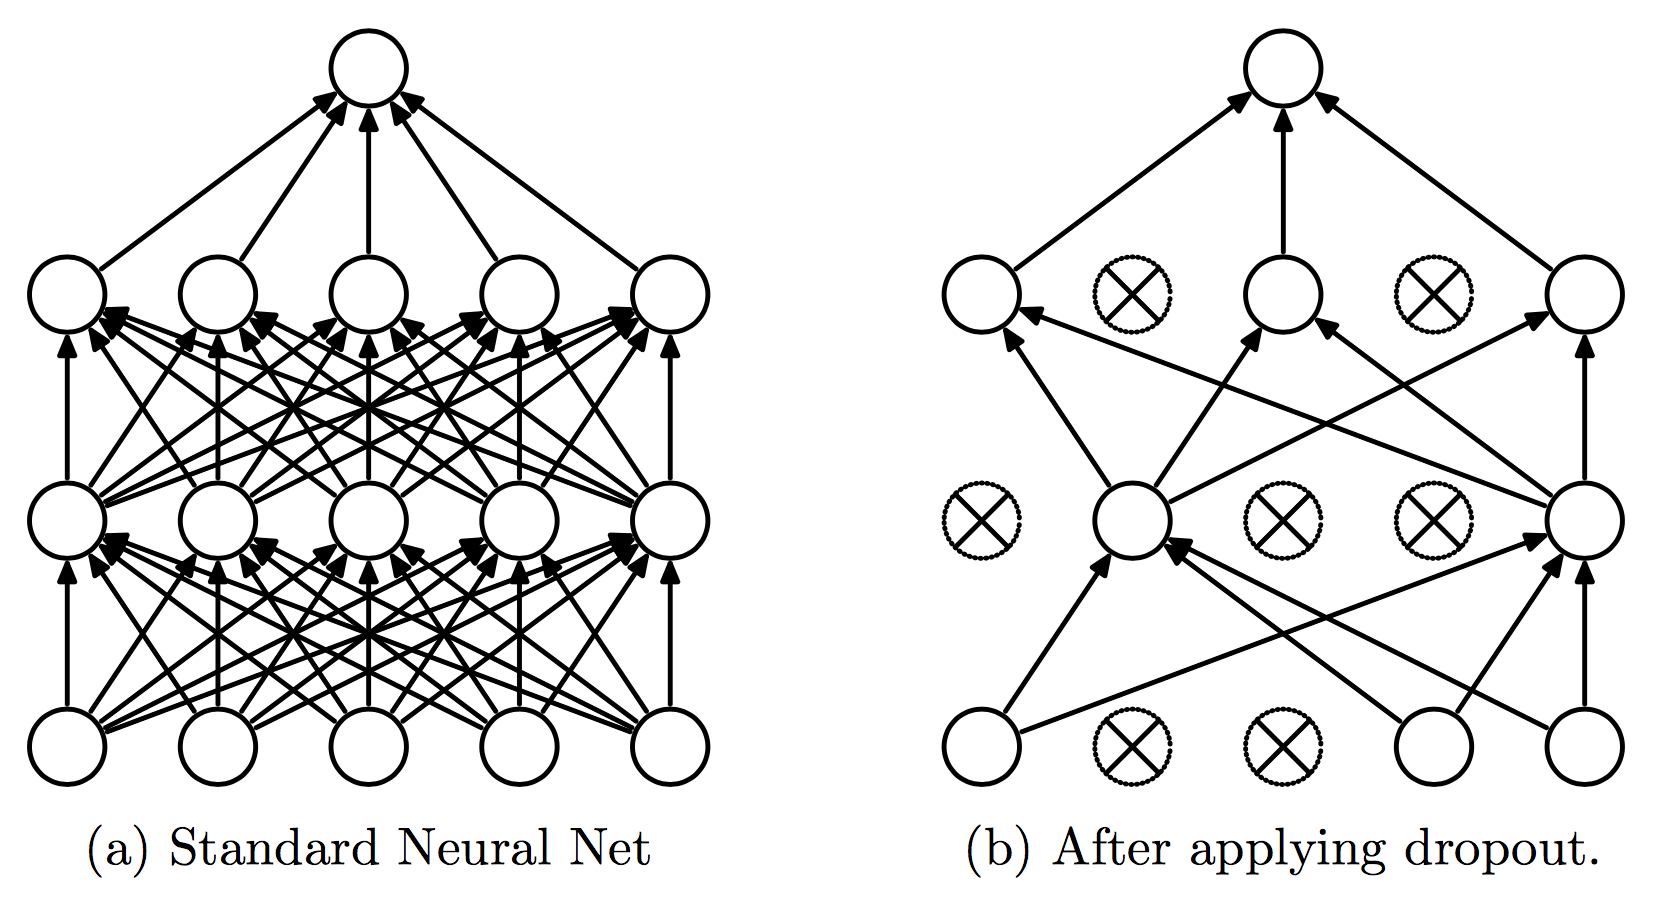
\includegraphics[width=0.8\textwidth]{figures/chapter-2/dropout.png}
		\caption{Dropout}\label{fig:dropout}
\end{figure}


% TODO Consider Dropconnect! Should I also include this? 


Figure \ref{fig:dropout} illustrates this concept: The original network (right side) is thinned out by the dropout resulting in the network on the right side. 

Today, dropout represents the de-facto standard for regularising neural networks and preventing them from overfitting. 


\subsection{Multi-Task Learning}
Neural networks are typically used to perform a single task that is formalised by minimising an appropriate objective function. However, sometimes it is desirable to train the network on multiple (related) tasks simultaneously. 
\begin{wrapfigure}{r}{0.4\textwidth}
	\caption{Multi-Task Learning}\label{fig:multitask-learning}   
	\centering
	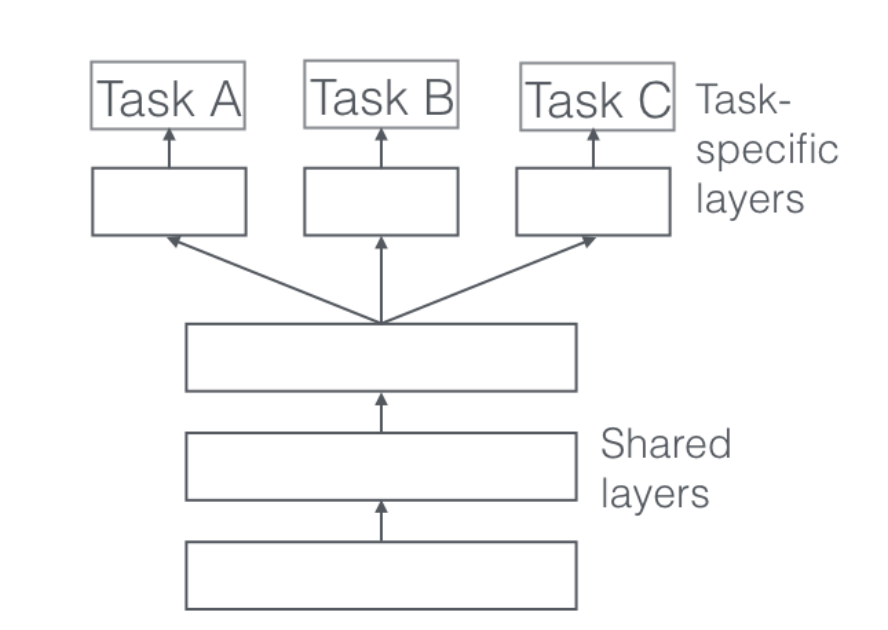
\includegraphics[width=0.4\textwidth]{figures/chapter-2/multitask-learning.png}
\end{wrapfigure}
As illustrated in figure \ref{fig:multitask-learning}, such a multi-task neural network is characterised by a number of layers that are shared among all tasks and a number of layers that are task-specific. Each task typically provides its own objective function which is optimised jointly with the objective functions of the other tasks. 
Multi-task learning can have a variety of desirable properties: Firstly, multi-task neural networks are typically less prone to overfitting as the shared layers have a regularising effect on the network forcing it to learn a shared representation among all tasks. In addition, they allow influencing the way a task is learnt on a more fine-grained level by introducing inductive biases that are provided by the other tasks. This means that we can make a primary task more inclined towards considering related sub-tasks. 
% CITE Inductive bias

As typical example for multi-task learning, we consider training a spam classifier for emails. Different users might have different distributions over the features of emails they receive due to factors such as language, contacts, age, and interests which can be conceptualised as a number of different tasks. Despite their differences these tasks are highly related allowing us to treat the classifier as a multitask-learning problem. Ideally, the shared layers would learn common concepts of the characteristics of spam emails whereas the individual task-specific layers would take into account the specific characteristics of the user. 

% ... "Bias-free learning is impossible; much of the power of an inductive learner follows directly from the power of its inductive bias [Mitchell 1980]."

% CITE Sebastian Ruder
% CITE http://www.cs.cornell.edu/~caruana/mlj97.pdf




\subsection{Model Selection and Architecture Learning} % TODO Is this the right expression? 
In section \ref{sec:nn-types} we described the three main types of neural networks which are each suitable for different kinds of tasks. However, even after deciding on a specific type, there are a number of architectural choices that are of great importance for the performance of the model. These architectural choices can be considered as model-level hyper-parameters that are typically defined a-priori and have to be chosen appropriately in addition to the hyper-parameters that were already discussed in the previous sections (e.g. learning rate $\alpha$, dropout probability $p$, activation function $f$, etc.). These following lists typical model-level hyper-parameters and how they might affect the network. 

\subsubsection{Model Hyperparameters}
\paragraph{i) Number of layers} The number of layers (or depth) of the network is a key design decision for the model's architecture and greatly influences its performance. In general, a higher number of layer results in a more complex model with high variance increasing its expressiveness and ability to capture complex non-linear dependencies. On the flip side, % TODO Can I say this? 
this leads to an increased probability of over-fitting the training data and therefore requires stronger regularisation. From a practical perspective, a higher number of layers will cause the training to more computationally expensive and requires more memory to store the trained parameters. Consequently, the choice reflects the classical tradeoff between bias and variance discussed in \ref{sec:regularisation} and depends on the amount of available data and computational resources. 

%| Number of Hidden Layers | Result |
%
%0 - Only capable of representing linear separable functions or decisions.
%
%1 - Can approximate any function that contains a continuous mapping
%from one finite space to another.
%
%2 - Can represent an arbitrary decision boundary to arbitrary accuracy
%with rational activation functions and can approximate any smooth
%mapping to any accuracy.
% TODO Point out that 2-4 layers almost always sufficient!
% TODO Should I include sample number and heuristics? 
% CITE some paper...

\paragraph{ii) Number of units per layer} In addition to the number of hidden layers, we need to decide on an appropriate number of units per hidden layer (network width). The decision follows a rationale similar to the number of layers: A high number of units per layer increase the variance of the model allowing it to accommodate more complex functions at the cost of more computational complexity and the danger of over-fitting.  


\subsubsection{Hyper-Parameter Optimisation}
In contrast to the ordinary parameters (weights and biases) of the model, hyper-parameters are typically not learnt during training but need to be chosen appropriate a-priori. However, there are three main techniques to derive suitable hyper-parameters:

\paragraph{i) Grid Search} The most basic form of finding appropriate hyper-parameters is to perform a \emph{grid search}. This means iteratively trying out a set of candidate values for each hyper-parameter and thereby exhaustively searching the space of potential hyper-parameters. After each iteration, the model is trained and then evaluated on a dedicated \emph{cross validation set}. % TODO Make sure I mention the splits somewheher!
While this approach is doable for a small space search space, it becomes computationally infeasible if the potential hyper-parameters (or their combinations) is large. 

\paragraph{ii) Random Search} An alternative to grid search that is computationally less expensive is \emph{random search}. Instead of trying every possible hyper-parameter in the search space exhaustively, this approach randomly samples hyper-parameters from the search space a fixed amount of times. 

\paragraph{iii) Bayesian Optimisation} Lorem ipsum dolor sit amet consectetur adipiscing elit eleifend massa ut, hac odio viverra feugiat vestibulum libero vulputate suspendisse facilisis, quam class molestie platea mollis turpis sem varius duis.


\subsubsection{Architecture Learning}
Nevertheless, a number of approaches to automatically deriving suitable architectures has been proposed by a concept called 

It is difficult to derive proper architecture. 
What's the right number of hidden layers? What's the right number of hidden units per layer, etc? 
Different approaches to architecture learning. Optimal Brain Surgeon/Damage. GridSearch, RandomSearch, Bayesian Optimisation.

%\subsection{Challenges}
%Computational complexity
%Lots of parameters (high memory)
%Lots of hyper-parameters 
%Low Understandability. Some people confuse softmax with confidence. 
%
%Lorem ipsum dolor sit amet consectetur, adipiscing elit mus neque montes, suspendisse et sociis vestibulum.


\section{Counterfactual Inference}
\subsection{Motivation}
Lorem ipsum dolor sit amet consectetur, adipiscing elit mus neque montes, suspendisse et sociis vestibulum.

\subsection{Formalisation}
Lorem ipsum dolor sit amet consectetur, adipiscing elit mus neque montes, suspendisse et sociis vestibulum.

\subsection{Counterfactual Inference vs. Supervised Learning}
Lorem ipsum dolor sit amet consectetur, adipiscing elit mus neque montes, suspendisse et sociis vestibulum.

\subsection{Propensity Score}
Lorem ipsum dolor sit amet consectetur, adipiscing elit mus neque montes, suspendisse et sociis vestibulum.

\subsection{Status Quo}
Lorem ipsum dolor sit amet consectetur, adipiscing elit mus neque montes, suspendisse et sociis vestibulum.

\subsection{Open Questions}
Lorem ipsum dolor sit amet consectetur, adipiscing elit mus neque montes, suspendisse et sociis vestibulum.

